\documentclass[a4paper]{article}
\usepackage[utf8]{inputenc}                   
\usepackage[french]{babel}
\usepackage{graphicx} 
\graphicspath{{./img/}}
\usepackage{amsmath, amssymb}
\usepackage{geometry}
\usepackage{url}
\usepackage[T1]{fontenc}
%\usepackage{minted}
\usepackage[perpage]{footmisc}
\usepackage[hidelinks]{hyperref}
\usepackage{caption}
\usepackage{subcaption}
\newcommand{\HRule}{\rule{\linewidth}{0.5mm}}

\author{Maël PAUL Maxime SALAND}
\begin{document}
%\title{\centering \textbf{Rapport Projet Sandwich}}
\begin{center}

\includegraphics[scale=0.15]{img/logo_EM_vertical.png}\\[1cm]
 \HRule \\[0.4cm]
{\huge \bfseries Rapport de Projet Sandwich \\[0.4cm]}
\HRule \\[1.5cm]
{\Large \textbf{Maël Paul} et \textbf{Maxime Saland}}\\[0.5cm]
{\Large Année universitaire 2021-2022}\\[1cm]
{\large Encadrant : Michaël Clément}
\hspace{0.5cm}
{\large Responsable projet : David Renault}

\end{center}

\thispagestyle{empty}

\newpage

\tableofcontents

\newpage
\section*{Introduction}
L'automate cellulaire est une grille de cellules dont chacune contient un état issu d'un ensemble fini et pouvant évoluer au cours du temps. L'état d'une cellule à une itération i dépend de l'état du voisinage\footnote{On considère ici qu'une cellule appartient à son propre voisinage.} de la cellule à l'itération i-1. Par conséquent, chaque état d'un automate cellulaire à une itération donnée est la résultante des états des cellules de cet automate à l'itération précédente. Un tel automate est capable de simuler des comportements complexes tels que des phénomènes physiques simplifiés comme du feu se propageant sur du bois ou l'écoulement d'un liquide, et ce, en partant d'un ensemble restreint de règles basiques.
Le projet Sandwich a pour objectif le développement  d'un ensemble de programmes informatiques permettant la modélisation d'un système au sein duquel des cellules évoluent au cours du temps. Le sujet consiste donc à développer des programmes permettant l'implémentation d'automates cellulaires en 2 dimensions. 
Dans un premier temps, nous commencerons par présenter le projet dans son ensemble en définissant ses objectifs, en passant par le contexte de sa réalisation et en concluant par sa structure. Dans un second temps, nous poursuivrons en traitant d'un objet particulièrement important durant le projet : la file. Enfin, nous terminerons par la réalisation des achievements.
\newpage

\section{Présentation du projet}
Le projet Sandwich étant un projet en binôme, il a nécessité différents outils ainsi qu'une organisation au sein de l'équipe afin de le réaliser. Cette première partie permet donc de traiter, non pas de la réalisation, mais des autres aspects essentiels au bon déroulement du projet. Dans un premier temps, nous traiterons de l'environnement de travail dans lequel s'est déroulé le projet. S'ensuivra d'une partie sur les objectifs du projet, tant pédagogique que les différents achievements ainsi que l'avancement de notre projet dans son état final. Puis, cette mise en contexte se conclura par la présentation de la structure du projet.
\vspace{0.3cm}

\subsection{Objectifs et avancements}
\vspace{0.1cm}
Le projet Sandwich étant le premier projet du cursus, il comporte des objectifs pédagogiques et des objectifs de "production".
On entend par objectifs pédagogiques les aspects entourant un projet qui sont nécessaires à sa réalisation. Le premier de ces objectifs était de travailler en équipe sur un même ensemble de fichiers/programmes. Le second objectif de ce premier projet était d'apprendre à travailler avec non pas un seul fichier, mais un ensemble de fichiers de codes sources et d'en-têtes, ayant chacun un rôle spécifique (détaillé à la partie~\ref{sec:ORGA_PROJ}). Ce travail à plusieurs sur une multitude de fichiers implique donc d'avoir une certaine rigueur dans la rédaction des programmes afin d'avoir des codes clairs et homogènes, ce qui constitue un troisième objectif.\\
\indent Outre ces objectifs, relevant plus de l'aspect pédagogique, demeurent les objectifs de réalisation liés au sujet. Le fil rouge de ce projet, évoqué en introduction, est la manipulation d'un automate cellulaire.
Dans le cadre de ce projet, nous sommes donc amenés à manipuler un \textbf{monde} en 2 dimensions au sein duquel évoluent un ensemble de \textbf{cellules}\footnote{L'affichage du monde correspond à une matrice 2D de pixels.}. Pour une itération donnée, chaque cellule est dans un unique état (par exemple 0) provenant d'un ensemble fini d'états possibles (par exemple \{0,1\}). À chaque itération (on peut parler ici d'image), chaque cellule peut changer ou non d'état en fonction de \textbf{règles} préétablies. Une règle est composée de 2 éléments : un motif et une transformation. Le motif est une séquence contenant l'état d'une cellule centrale (sujette à un changement d'état) ainsi que les états de ses cellules voisines. La transformation va quant à elle spécifier l'état que va prendre la cellule centrale si le motif est reconnu. Par exemple, soit une règle indiquant qu'une cellule marron, symbolisant du bois, entourée de cellules rouges, symbolisant du feu, s'enflamme (la cellule devient rouge). Cette règle aura donc pour motif une cellule centrale marron dont les cellules voisines sont intégralement rouges, et pour transformation la couleur rouge.\\
\indent Partant de ce fil rouge, les achievements traitent des différents aspects et problèmes liés à l'implémentation d'un automate cellulaire. Dans notre cas, nous avons complété les achievements 0 (jeu de la vie), 1 (multicoloritude) et 2 (simulation de particules). L'ensemble des achievements suivant n'ont pas été traités et ne seront donc pas évoqués dans ce rapport.


\subsection{Cadre de travail}
\vspace{0.1cm}
Ce premier projet a été l'occasion de découvrir le travail en équipe, de taille modeste, sur un même code. Travailler en binôme implique donc de s'imposer des contraintes afin de pouvoir travailler efficacement et surtout afin d'éviter de se gêner mutuellement dans son travail. Dans cette optique de travail à plusieurs, il a alors été nécessaire d'établir dès le commencement, une convention pour la rédaction des futurs programmes. Cette étape est nécessaire, car même si une convention avait été vue lors de notre apprentissage du langage C, il y a presque toujours des différences dans la façon dont chacun écrit du code. Avoir une convention commune permet donc d'avoir du code cohérent dans sa forme, facilitant notamment la relecture du code écrit par son binôme.\\
\indent Comme dans la plupart des projets actuels d'informatique, le logiciel de versionnage Git a été utilisé afin de travailler en parallèle sur les différents programmes. Le projet a ainsi été l'occasion de découvrir Git et d'apprendre à l'utiliser correctement (gestion des conflits, retour sur une version précédente, etc.).\\
\indent Enfin, le projet contient une multitude de fichiers devant être compilés. Cette étape de compilation est répétée de nombreuses fois lors du projet et devient rapidement redondante. C'est pourquoi un fichier Makefile a été utilisé afin d'entre autres simplifier la compilation des différents fichiers afin de produire l'exécutable principal ainsi que celui de test.

\subsection{Organisation du projet}\label{sec:ORGA_PROJ}
\vspace{0.1cm}
Afin d'avoir un projet structuré, ce dernier est constitué d'un ensemble de fichiers ayant chacun un rôle qui leur est propre. La plupart des fichiers dépendent d'un ou plusieurs fichiers d'en-tête/.h (cf. figure \ref{fig:diag} ci-dessous).

\begin{figure}[ht]
    \centering
    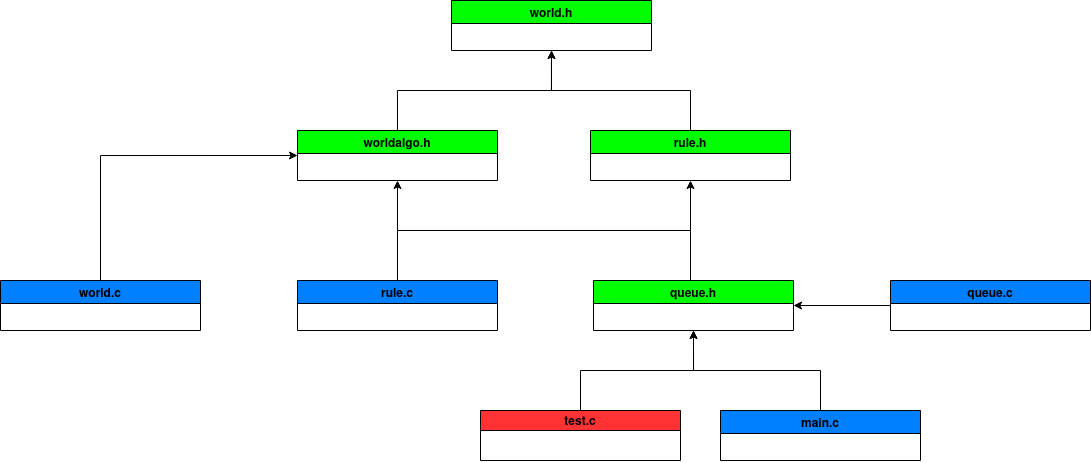
\includegraphics[scale=0.4]{img/diagramme_dependance.png}
    \caption{Diagramme des dépendances}
    \label{fig:diag}
\end{figure}

Comme le montre le schéma précédent, le projet est composé de fichiers d'en-têtes (d'extension .h) et de fichiers contenant le code source (d'extension .c).\\
Le projet peut être décomposé en 3 objets principaux : les règles, le monde et la file.
Chacun de ces objets est implémenté dans un fichier différent. Tout d'abord, les règles sont définies dans le fichier rule.c contenant la structure des règles et l'ensemble des fonctions associées. Similairement, le monde est implémenté au sein du fichier world.c et la file dans queue.c. La boucle principale calculant les images successives du monde se trouve dans le fichier main.c et les tests sont quant à eux effectués dans le fichier test.c.\\
\\
\indent La forme du projet ayant été désormais expliquée dans son ensemble, nous pouvons passer  à sa réalisation en commençant avec la structure de file.

\newpage

\section{La file}\label{sec:file}
En informatique, une file est une structure de données basée sur le principe FIFO (First In, First Out), ce qui signifie que les premiers éléments ajoutés à la file seront les premiers à en être retirés.\\ 
\indent Les cellules étant évaluées une par une, il ne faut pas appliquer les transformations après chaque évaluation, mais le faire une fois que l'ensemble des cellules ont été évaluées. Cette contrainte est nécessaire, car sans elle le calcul du monde à l'itération i+1 serait erroné étant donné que celui-ci ne résulterait pas des états des cellules à l'itération i. C'est pourquoi une file est implémentée afin de stocker au fur et à mesure les transformations puis de les appliquer en défilant ses éléments. L'implémentation de la file s'est faite par l'intermédiaire de deux fichiers : queue.h et queue.c. Le fichier queue.h contient les includes, constantes, définitions de structures et primitives de fonctions nécessaires pour pouvoir utiliser la file dans le fichier main.c. Le fichier queue.c contient quant à lui le code des différentes fonctions qui permettent l'utilisation de la file, comme l'ajout et la suppression d'un élément.

\subsection{queue.h}
Le fichier queue.h contient les includes des fichiers worldalgo.h et rule.h (cf. figure \ref{fig:diag}), cela permet d'avoir accès à la structure des règles (\texttt{struct rule}) ainsi qu'aux constantes {\small WIDTH} et {\small HEIGHT} qui serviront pour définir les deux structures nécessaires à l'utilisation de la file.
\\\indent La première structure est celle des éléments de la file:
\begin{figure}[htb]
    \centering
    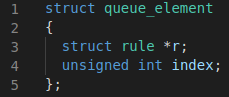
\includegraphics[scale=0.8]{img/queue_element.png}
\end{figure}
\\\indent Le premier champ \texttt{r} est un pointeur vers une règle car le fichier rule.h nous permet seulement d'avoir accès au type incomplet \texttt{struct rule}. Le deuxième champ \texttt{index} est l'indice de la cellule du monde sur laquelle la règle pointée s'applique.
\\\indent La deuxième structure est celle de la file:
\begin{figure}[h]
    \centering
    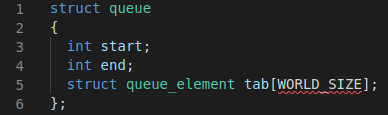
\includegraphics[scale=0.8]{img/queue.png}
\end{figure}
\\\indent Le premier champ \texttt{start} est l'indice du premier élément de la file. Le deuxième champ \texttt{end} est l'indice de la première case vide dans la file. Le champ \texttt{end} a la priorité sur \texttt{start}, c'est-à-dire que si \texttt{start = end} alors la file est vide. Le troisième champ est un tableau de \texttt{queue\_element} qui représente la file, ce tableau est de taille {\small WORLD\_SIZE}, constante définie comme étant égale à {\small WIDTH $\times$ HEIGHT}, ce qui est la taille du monde. En effet, la façon dont nous avons implémenté nos achievements fait que, pour une cellule donnée du monde, il y a au plus une règle qui s'applique sur cette cellule, il y a donc au maximum {\small WORLD\_SIZE} transformations à effectuer.

\subsection{queue.c}
Le fichier queue.c contient l'include du fichier queue.h, ainsi que le code des différentes fonctions permettant de manipuler la file.
D'un point de vue algorithmique, toutes les fonctions de manipulation de la file et de ses éléments s'effectuent en temps constant.
Les deux opérations majeures concernant la file sont l'ajout et la suppression d'un élément.
\\Exemple de file:
\\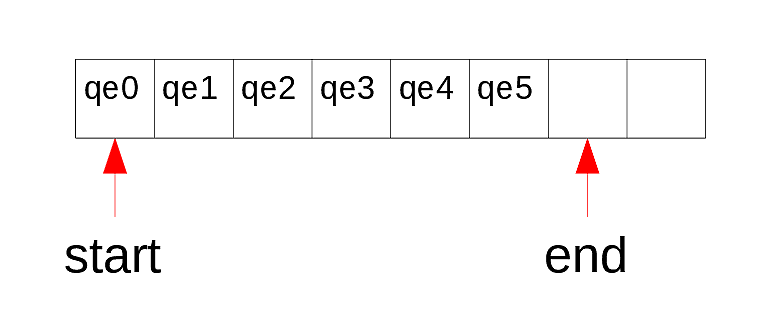
\includegraphics[scale=0.35]{img/file.png}
\\Ajout d'un élément \textbf{x}:
\\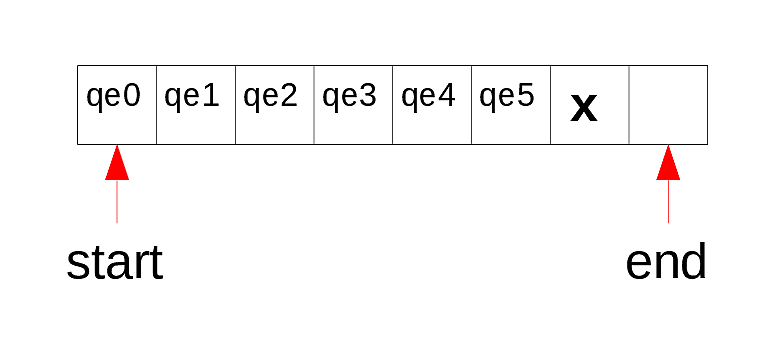
\includegraphics[scale=0.35]{img/file1.png}
\\Suppression d'un élément (l'élément supprimé, ici \texttt{qe0}, est retourné) :
\\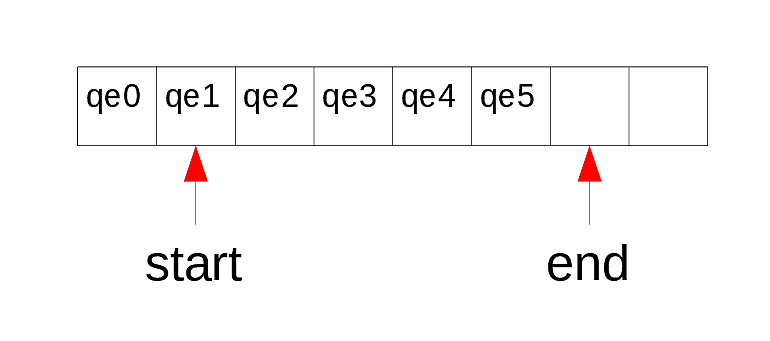
\includegraphics[scale=0.35]{file2.png}
\\L'utilisation des indices \texttt{start} et \texttt{end} permet de manipuler la file en temps constant par simple décalage de ces deux indices.

\subsection{Tests}
Dans le fichier test.c, nous avons testé le bon fonctionnement de la file et plus particulièrement les fonctions \texttt{queue\_append} et \texttt{queue\_pop}. Nous avons tout d'abord essayé d'ajouter un nombre plus grand d'éléments que la taille de la file pour vérifier que l'on ne puisse plus ajouter d'éléments dans celle-ci lorsque sa capacité maximale est atteinte. Nous avons ensuite défilé au-delà de la taille maximale de la file afin de s'assurer que l'élément retourné par \texttt{queue\_pop} est l'élément vide lorsque la file est vide.

\newpage
\section{Réalisation des achievements}
Le projet est découpé en plusieurs grandes étapes (achievements) plus ou moins dépendantes des étapes qui les précèdent. La partie ci-après traite de la réalisation des 3 achievements que nous avons réalisé lors du projet.
\subsection{Le jeu de la vie} \label{sec:GOL}
Le jeu de la vie est un automate cellulaire créé en 1970 par le mathématicien britannique John Horton Conway. Dans cet automate, les cellules ne peuvent avoir que 2 états possibles : vivant ou mort. De plus, les règles du jeu de la vie sont très simples :
\begin{itemize}
    \item une cellule morte entourée de 3 vivantes devient vivante
    \item une cellule vivante entourée de 0, 1 ou 4 et plus cellules vivantes devient morte
\end{itemize}
Le premier achievement du projet (version de base) porte sur l'implémentation du jeu de la vie. Étant donné que le passage de la définition en langage naturel à l'implémentation via un langage informatique (C dans notre cas) n'est pas (encore) faisable automatiquement, plusieurs problèmes se posent. En effet, le jeu de la vie est un automate cellulaire correspondant à un monde rempli de cellules dont les états sont régis par des règles. L'implémentation du jeu de la vie a donc nécessité d'implémenter un monde, des règles et des fonctions permettant de manipuler ces objets.
\subsubsection{Le monde}
\indent L'implémentation du monde est commune à l'ensemble des achievements que nous avons réalisé lors du projet. Le premier problème, bien que mineur, est l'impossibilité d'avoir des structures de données en plusieurs dimensions en C alors que le monde devant être manipulé est en 2 dimensions. Pour pallier ce problème, le monde est implémenté comme un tableau unidimensionnel. Afin de pouvoir manipuler le monde comme une matrice en 2 dimensions, la fonction \texttt{coord\_to\_idx} a été développée. Cette fonction calcul l'indice dans le monde à partir de la largeur du monde ainsi que des coordonnées de la cellule via la formule \texttt{\(\text{indice} = \text{largeur}\times \text{coord\_ligne} + \text{coord\_col}\)}. Une fois la structure du monde implémentée, il est nécessaire de pouvoir générer aléatoirement un monde faisant office d'état initial pour le jeu de la vie. Pour ce faire, il faut d'abord définir les états qu'une cellule peut prendre. Dans le jeu de la vie, une cellule est soit morte, soit vivante, ce qu'on peut représenter par 0 (morte) et 1 (vivante). Néanmoins, le monde doit être affiché via un exécutable prenant en entrée une matrice d'entiers représentant chacun une couleur. Cet encodage des couleurs par des entiers complexifie la lecture du code. En effet, bien que le noir soit reconnaissable, car représenté par 0, le blanc est quant à lui représenté par 16 777 215 (ce qui n'est pas très évocateur). De plus, les prochains achievements du projet utilisent plusieurs couleurs ce qui rendrait le code illisible tel quel. Pour pallier cela, on utilise une énumération nous permettant de créer une "liste" d'entiers nommés. On peut ainsi remplacer, grâce à une énumération, 16 777 215 par {\small WHITE} et 0 par {\small BLACK}.
Comme précisé dans la partie \ref{sec:ORGA_PROJ}, la génération du monde est gérée dans le fichier world.c (cf. ci-après pour le programme de génération aléatoire\footnote{Les programmes ci-après ne sont pas rédigés exactement pareil dans notre projet. Il s'agit ici d'un pseudo-code C montrant surtout les aspects importants de ces fonctions.}).
Dans ce fichier, la génération est composée d'une fonction principale \texttt{world\_init\_gol} qui va remplir chaque cellule du monde en appelant la fonction auxiliaire \texttt{color\_cell} dont le code est visible ci-après.
\begin{figure}[htb]
    \centering
    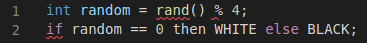
\includegraphics[scale=0.8]{img/WB.png}
\end{figure}
\\Cette fonction retourne aléatoirement, et selon une certaine proportion (\(\frac{1}{4}\) dans notre cas), la couleur blanche ou noire. Pour ce faire elle génère un entier aléatoire qu'on restreint à l'intervalle [\![0 ; 3]\!] à l'aide d'un modulo. Il est donc possible de générer des mondes avec plus ou moins de cellules vivantes. La figure~\ref{fig:world_gol} ci-dessous montre un exemple de monde généré par un appel de \texttt{world\_init}.
\begin{figure}[htb]
    \centering
    
\includegraphics[scale=0.3]{img/monde_gol.png}
    \caption{Monde généré par \texttt{world\_init}}
    \label{fig:world_gol}
\end{figure}
\\
\indent Le monde étant opérationnel, il reste à implémenter la partie la plus volumineuse du projet : les règles.

\subsubsection{Les règles}
Bien que les règles du jeu de la vie soient peu nombreuses à énoncer, leur nombre augmente considérablement lorsqu'on souhaite les traduire en C. En effet, une règle correspond à un motif et à une transformation. Chaque motif correspond à un carré de 3 par 3 cellules et chaque cellule peut prendre un état parmi un ensemble de 2 états, il y a donc 512 (= \(2^9\)) motifs possibles. En outre, l'implémentation du jeu de la vie requiert d'initialiser 512 règles différentes. Ce nombre conséquent de règles incite fortement à concevoir une structure de règle permettant d'initialiser les règles via une boucle. Les règles suivent toutes la structure suivante :
\begin{figure}[h]
    \centering
    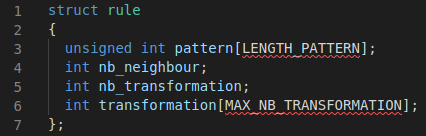
\includegraphics[scale=0.8]{img/rules1.png}
\end{figure}
\\\indent Chaque règle comporte donc un motif représenté par le tableau d'entiers positifs \texttt{pattern} de taille {\small LENGTH\_PATTERN} fixée à 9, un champ \texttt{nb\_neighbour} correspondant au nombre de cellules voisines vivantes, un champ \texttt{nb\_transformation} indiquant le nombre effectif de transformations\footnote{La constante {\small MAX\_NB\_TRANSFORMATION} est utilisée pour définir la taille du tableau des transformations, mais le véritable nombre de transformations d'une règle est indiqué par le champ \texttt{nb\_transformation}.}, et un tableau \texttt{transformation}, contenant la (les) transformation(s) possible(s) pour ledit motif, et de taille {\small MAX\_NB\_TRANSFORMATION}, le nombre maximal de transformations possibles pour une cellule, que nous avons choisi de fixer à 5. L'ensemble des règles sont stockées dans un tableau global \texttt{rules} de taille {\small NB\_RULE} (= 512) permettant l'accès aux règles depuis le fichier main.c (contenant l'algorithme calculant les images successives du monde).\\
\indent La forme des règles étant désormais établie, il reste à en établir le fond. L'initialisation des 512 règles du jeu de la vie est assuré par la fonction \texttt{rules\_init\_gol}, ainsi que les 3 fonctions auxiliaires \texttt{num\_color\_match}, \texttt{array\_cpy} et \texttt{set\_transformation}. Hormis le nombre de transformations, le remplissage des champs de la règle doit être effectué dans l'ordre. En effet, la transformation dépend de la couleur de la cellule centrale (et donc du motif de la règle) ainsi que du nombre de cellules voisines vivantes (champ dépendant lui aussi du motif). En outre, la fonction va premièrement s'occuper de générer le motif, puis de compter le nombre de cellules voisines en vie et enfin affecter la transformation. La génération des motifs est visible dans le code ci-dessous :
\begin{figure}[htb]
    \centering
    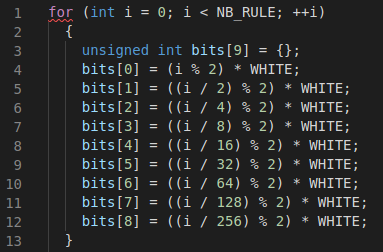
\includegraphics[scale=0.8]{img/boucle.png}
\end{figure}
\\\indent Cette boucle d'apparence peu accueillante génère l'ensemble des tableaux binaires de longueur 9. Les valeurs étant des 0 et des 1, les motifs obtenus ne correspondent pas à ceux trouvables dans le monde (car les cellules valent soit 0, soit 16 777 215). On multiplie de ce fait par {\small WHITE} (= 16 777 215) pour avoir les motifs en noir et blanc.
Une fois le motif obtenu, le nombre de cellules voisines vivantes est affecté via la fonction \texttt{nb\_color\_match} (qui effectue un simple comptage à partir du motif). Enfin, la transformation est décidée avec la fonction \texttt{set\_transformation} qui correspond à une traduction en C des règles du jeu de la vie (cf. code ci-dessous).
\begin{figure}[htb]
    \centering
    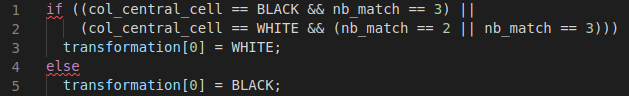
\includegraphics[scale=0.8]{img/nb_match.png}
\end{figure}
\\\indent Les règles étant désormais initialisées, il faut être capable de déterminer si pour une cellule et une règle données, il y a correspondance entre la cellule et la règle (ou plutôt entre le voisinage de la cellule et le motif de la règle). Pour ce faire, il faut donc récupérer les états du voisinage de la cellule. Cependant, les états des cellules sont stockés dans un tableau unidimensionnel ce qui veut donc dire que les cellules voisines ne sont pas adjacentes à la cellule. De plus, le monde sur lequel nous travaillons est torique, par conséquent certaines cellules "voisines" sont en vérité très distantes dans le tableau de la structure du monde comme l'illustre la figure~\ref{fig:torique} ci-après.\\
\begin{figure}[htb]
    \centering
    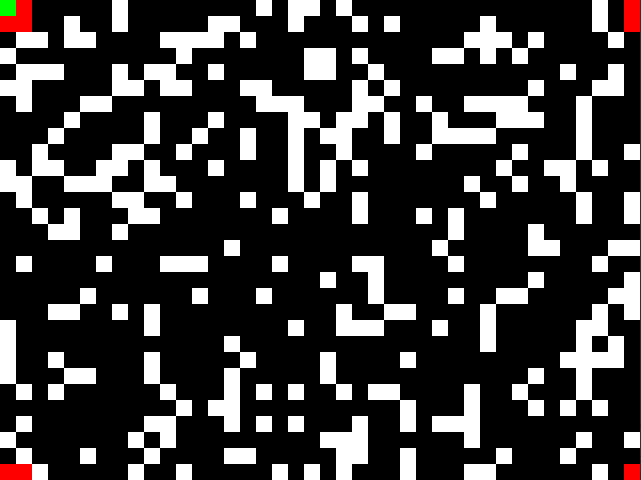
\includegraphics[scale=0.3]{img/torique.png}
    \caption{La première cellule du monde (vert) et ses voisines (rouge)}
    \label{fig:torique}
\end{figure}
\newpage
Les indices du voisinage vont être calculés à partir des coordonnées de la cellule centrale via la fonction \texttt{surrounding\_idx} (cf. ci-dessous).
\begin{figure}[htb]
    \centering
    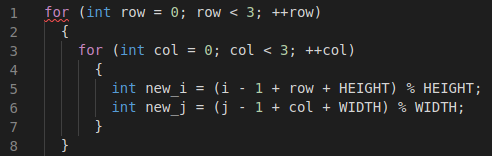
\includegraphics[scale=0.8]{img/indice.png}
\end{figure}
\\\indent Les formules ci-dessus permettent d'obtenir les coordonnées dans un carré de taille 3 par 3. Par exemple, lorsque \texttt{row} et \texttt{col} sont à 0 (premier tour de boucle), on va calculer les indices du voisin situé en haut à gauche. Puis, lorsque \texttt{col} s'incrémente, on calcule les coordonnées du voisin juste au-dessus, et ainsi de suite jusqu'à ce que l'ensemble du voisinage ait été parcouru. Pour la première cellule (de coordonnées nulles), les coordonnées (ligne puis colonne) du voisin supérieur gauche sont {\small (29, 39)\footnote{new\_i = \((0-1+0+30)\%30 = 29\) et new\_j =\((0-1+0+40)\%40 = 39)\)}} ce qui correspond bel et bien aux coordonnées de la dernière cellule du monde (cf. figure~\ref{fig:torique}). Une fois ce problème résolu, la fonction \texttt{rule\_match}, chargée d'évaluer la correspondance entre cellule et règle, ne présente plus de véritable problématique. La fonction va pouvoir simplement récupérer les valeurs du voisinage et les comparer avec celles du motif.

\subsubsection{Le calcul des itérations}
La file, le monde et les règles étant tous désormais implémentés avec pour chacun un ensemble de fonctions permettant leur manipulation, il reste la dernière étape consistant à combiner ces éléments dans un algorithme principal produisant les différentes itérations du monde. Cette ultime étape se passe dans le fichier main.c. L'algorithme principal calculant les différentes générations (images) du monde va pour chaque cellule et pour chaque règle vérifier s'il y a correspondance via la fonction \texttt{rule\_match}. En cas de correspondance, la règle (ou plutôt son adresse) est ajoutée à la file. Puis, les transformations sont appliquées à chaque cellule en défilant les éléments de la file et en appelant la fonction \texttt{world\_apply\_rule}. La boucle principale itérant sur \emph{n} images ainsi que sur l'ensemble des cellules et sur chacune des règles, le nombre de boucles est \(\text{nb\_cellules} \times \text{nb\_règles} \times \text{nb\_images}\). À chaque tour de boucle, on appelle \texttt{rule\_match} et \texttt{queue\_append} qui s'effectuent en temps constant (\texttt{rule\_match} compare toujours deux tableaux de 9 éléments). Le parcours de la file et l'affichage du monde étant  négligeable par rapport à la boucle parcourant l'ensemble des cellules et des règles, on conclut que la complexité temporelle du programme principal (fonction main du fichier main.c) est O(\(\text{nb\_cellules} \times \text{nb\_règles} \times \text{nb\_images}\)).
\\
\indent Cette première partie du projet a permis d'implémenter un premier automate cellulaire, en particulier celui du jeu de la vie. Cependant, dans cette première version, chaque cellule ne peut avoir qu'une unique transformation possible par itération. L'achievement numéro 1 intitulé \emph{multicoloritude} porte sur cet aspect et propose de permettre aux cellules d'avoir plusieurs transformations possibles.

\subsection{Le jeu de la vie en couleur}
Pour cet achievement, nous avons décidé de reprendre l'automate du jeu de la vie et d'attribuer aux cellules vivantes 3 couleurs supplémentaires (ajoutées à l'enum color) : le bleu, le rouge et le vert. Ce changement, bien que mineur, va nécessiter de réviser les fonctions développées pour le monde et les règles. Cependant, l'ajout de nouvelles couleurs ne nécessite pas de remise à niveau pour la file.
Pour le monde comme pour les règles, le fait que les cellules vivantes puissent être représentées par 4 couleurs peut causer une perte de performances considérable, car il y aurait désormais 1 953 125 (\(= 5^9\)) règles différentes. C'est pourquoi on ajoute une couleur "neutre" dans l'énumération des couleurs, n'ayant pas pour but d'être affichée, mais de représenter l'ensemble des couleurs désignant une cellule vivante (bleu, blanc, rouge et vert).

\subsubsection{Génération d'un monde multicolore}
Jusqu'à présent, le monde était généré uniquement en noir et blanc via la fonction \texttt{world\_init\_gol} qui remplissait chaque cellule en appelant \texttt{color\_cell}. Afin de réutiliser la fonction \texttt{color\_cell}, celle-ci ne retournera plus du blanc une fois sur quatre mais la nouvellement créée couleur neutre. Toutefois, la couleur neutre n'est pas pensée pour être affichée et indique uniquement que la cellule est vivante. Par conséquent, on n'affecte plus directement la valeur de retour de \texttt{color\_cell} aux cellules. Au lieu de ça, on teste la valeur retournée par \texttt{color\_cell} : si c'est neutre, une couleur est choisie aléatoirement dans un tableau contenant les 4 couleurs possibles pour une cellule vivante, sinon, la cellule sera noire.
La figure~\ref{fig:world_col} ci-dessous permet de voir un monde issu de cette génération multicolore.

\begin{figure}[htb]
    \centering
    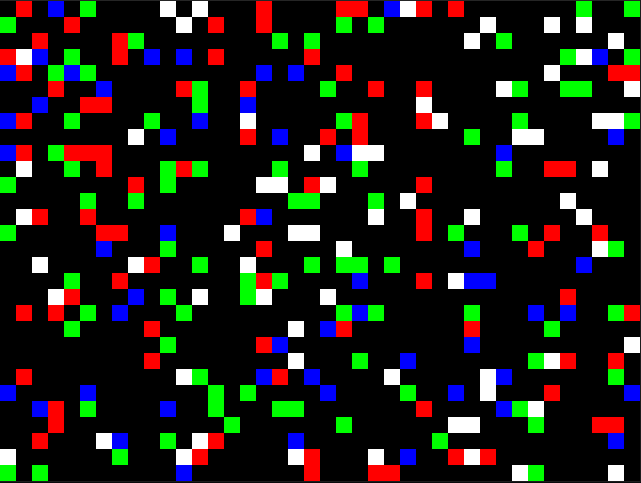
\includegraphics[scale=0.25]{img/monde_couleur.png}
    \caption{Monde multicolore généré par \texttt{world\_init}}
    \label{fig:world_col}
\end{figure}

\subsubsection{Modification des fonctions de règles}
Du côté des règles, les modifications ne sont pas trop gênantes. Dans la fonction \texttt{rules\_init}, plusieurs changements sont nécessaires afin d'initialiser correctement les motifs. Premièrement, le blanc est remplacé par la couleur neutre lors de la génération du motif. De plus, le champ indiquant le nombre de transformations est désormais à 4 (car une cellule vivante peut être représentée par 4 couleurs). Par conséquent, \texttt{set\_transformation} qui affectait noir ou blanc au tableau des transformations doit dorénavant affecter les 4 couleurs "vivantes" ou 4 fois la couleur noire. La modification des motifs implique de modifier \texttt{rule\_match} car les valeurs prises par les cellules (bleu, blanc, rouge, vert ou noir) ne sont plus comparables avec celles des motifs (neutre ou noir). Afin de résoudre ce problème, lorsque \texttt{rule\_match} récupère les couleurs, si la couleur est l'une des 4 couleurs "vivantes" alors on stocke dans le tableau du voisinage la couleur neutre, rendant de nouveau comparable le voisinage avec le motif d'une règle.

\subsection{Le sable}
L'achievement 2 vise à permettre aux cellules de se déplacer (comme des particules). Nous avons décidé de simuler du sable chutant et glissant, ainsi que de la roche. Dans cet achievement, nous ne gérons pas les conflits qu'il peut y avoir dans le cas où deux, ou plus, grains de sable se déplace vers une même cellule. Il y a donc superposition des grains de sable qui fusionnent, causant donc une perte de cellules de sable.  

\subsubsection{Ajout de nouvelles couleurs}
Pour représenter l'écoulement du sable, nous avons tout d'abord dû ajouter de nouvelles couleurs dans le \texttt{enum\_color}. Le sable sera représenté par du jaune, la roche par du gris et le vide par du noir. Des couleurs similaires à la couleur neutre (vide, roche, sable) sont ajoutées afin de pouvoir limiter le nombre de motifs à générer : le non-noir (sable et roche) et le non-gris (vide et sable).

\subsubsection{Le monde}
L'implémentation du monde est la même que celle du jeu de la vie. Le monde est initialisé à l'aide des fonctions \texttt{color\_cell} et \texttt{world\_init\_particule}. Le monde est tout d'abord initialisé avec un quart de sable et le reste du monde est vide (= noir). Puis, le bas du monde est défini comme de la roche parsemée de quelques trous afin que le sable puisse s'écouler continuellement. On ajoute aussi quelques pentes et plateformes de roche afin de pouvoir illustrer l'ensemble des comportements du sable. La figure~\ref{fig:world_sand} ci-dessous illustre la nouvelle génération de monde.
\newpage
\begin{figure}[htb]
    \centering
    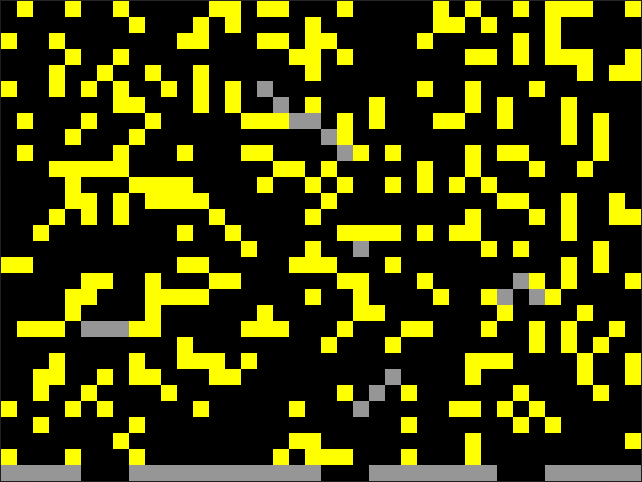
\includegraphics[scale=0.3]{img/world_sand.png}
    \caption{Monde initialisé par \texttt{world\_init}}
    \label{fig:world_sand}
\end{figure}

\subsubsection{Ajout de nouveaux champs dans la struct rule}
Pour implémenter les règles qui définissent le mouvement du sable, nous avons repris la structure des règles du jeu de la vie. Cependant, pour gérer le déplacement des grains de sable, il a fallu modifier cette structure de manière à pouvoir stocker les valeurs de déplacement horizontal et vertical d'un grain de sable dans les règles. Deux nouveaux champs \texttt{dx} et \texttt{dy} ont donc été ajoutés.
\begin{figure}[htb]
    \centering
    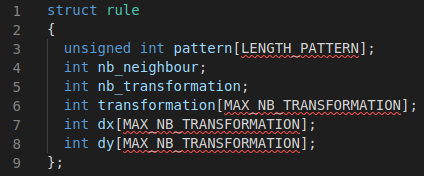
\includegraphics[scale=0.7]{img/rules2.png}    
\end{figure}
\\\indent Le tableau \texttt{dx} (respectivement \texttt{dy}) est un tableau d'entiers représentant le déplacement selon l'axe horizontal (respectivement l'axe vertical) du grain de sable associé à la transformation ayant le même indice dans le tableau \texttt{transformation}. Pour un indice donné \textbf{i}, si \textbf{dx[i] > 0} alors le déplacement s'effectue vers la droite, si \textbf{dx[i] < 0} alors le déplacement s'effectue vers la gauche, et si \textbf{dx[i] = 0} alors il n'y a pas de déplacement selon l'axe \textbf{x}. De même, si \textbf{dy[i] > 0} alors le déplacement s'effectue vers le bas, car nous représentons la chute du sable, si \textbf{dy[i] < 0} alors le déplacement s'effectue vers le haut, et si \textbf{dy[i] = 0} alors il n'y a pas de déplacement selon l'axe \textbf{y}. Le champ \texttt{nb\_neighbour} n'est quant à lui pas utilisé. Les autres champs gardent la même signification que pour le jeu de la vie.

\subsubsection{Les règles}
On utilise de nouveau le tableau global \texttt{rules} de taille {\small NB\_RULE} pour stocker les différentes règles définissant les déplacements possibles pour le sable. Pour cet achievement, seulement 6 règles sont nécessaires donc {\small NB\_RULE = 6}.
Le travail d'initialisation des 6 règles du jeu de la vie est assuré par la fonction \texttt{rules\_init\_particule} et la fonction auxiliaire \texttt{array\_cpy}, comme le montre le code ci-dessous initialisant la règle indiquant qu'un grain de sable ayant du vide en dessous chute.
\newpage
\begin{figure}[htb]
    \centering
    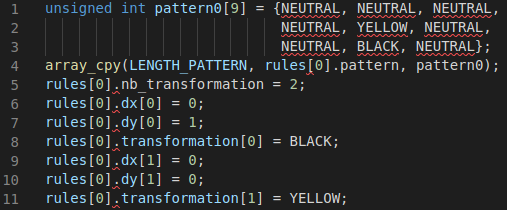
\includegraphics[scale=0.7]{img/pattern.png}
\end{figure}
\indent On remarque ici que les tableaux \texttt{dx}, \texttt{dy} et \texttt{transformation} ont 2 indices. Le premier élément de ce tableau correspond à la case de départ (là où se trouve le sable avant de chuter). Comme le sable (donc la cellule) chute, on indique \texttt{dx[0]=0} (aucun mouvement horizontal) et \texttt{dy[0]=1} (déplacement vers le bas). De plus, comme le sable chute, la cellule devient vide, c'est pourquoi sa transformation est du noir. Réciproquement, le second indice des tableaux \texttt{dx}, \texttt{dy} et \texttt{transformation} correspond à la case d'arrivée du grain de sable. Comme le sable arrive sur la case, la transformation est donc jaune. Comme il s'agit de la case d'arrivée, on fixe les déplacements de cette cellule à 0.
\\
\begin{figure}[!h]
    \centering
    \begin{subfigure}[t]{0.17\textwidth}
        
\includegraphics[width=\textwidth]{img/rule10.png}
        %subcaption{Pattern règle numéro 1} 
    \end{subfigure}
    \hfill
    \begin{subfigure}[t]{0.17\textwidth} 
        
\includegraphics[width=\textwidth]{img/fleche3.png} 
        %%subcaption{}
    \end{subfigure}
    \hfill
    \begin{subfigure}[t]{0.17\textwidth}
        
\includegraphics[width=\textwidth]{img/rule11.png}
        %subcaption{Déplacement vers le bas}
    \end{subfigure}
    \caption{Règle numéro 1 - Déplacement vers le bas}
\end{figure}

Les 5 autres règles sont implémentées de la même façon que pour la règle numéro 1. Elles permettent de décrire tous les motifs poussant un grain de sable à se déplacer et donc tous les déplacements possibles pour un grain de sable. Elles sont représentées ci-dessous.
\\
\begin{figure}[!h]
    \centering
    \begin{subfigure}[t]{0.17\textwidth}
        
\includegraphics[width=\textwidth]{img/rule20.png}
        %subcaption{Pattern correspondant à la règle numéro 2} 
    \end{subfigure}
    \hfill
    \begin{subfigure}[t]{0.17\textwidth}
        
\includegraphics[width=\textwidth]{img/fleche3.png}
        %subcaption{Mouvement numéro 1 (déplacement en bas à gauche)}
    \end{subfigure}
    \hfill
    \begin{subfigure}[t]{0.17\textwidth}
        
\includegraphics[width=\textwidth]{img/rule21.png}
        %subcaption{Mouvement numéro 2 (déplacement en bas à droite)}
    \end{subfigure}
    \caption{Règle numéro 2 - Déplacement en bas à gauche}
\end{figure}

\newpage
\begin{figure}[!h]
    \centering
    \begin{subfigure}[t]{0.17\textwidth}
        
\includegraphics[width=\textwidth]{img/rule20.png}
        %subcaption{Pattern correspondant à la règle numéro 2} 
    \end{subfigure}
    \hfill
    \begin{subfigure}[t]{0.17\textwidth}
        
\includegraphics[width=\textwidth]{img/fleche3.png}
        %subcaption{Mouvement numéro 1 (déplacement en bas à gauche)}
    \end{subfigure}
    \hfill
    \begin{subfigure}[t]{0.17\textwidth}
        
\includegraphics[width=\textwidth]{img/rule22.png}
        %subcaption{Mouvement numéro 2 (déplacement en bas à droite)}
    \end{subfigure}
    \caption{Règle numéro 2 - Déplacement en bas à droite}
\end{figure}

\begin{figure}[!h]
    \centering
    \begin{subfigure}[t]{0.17\textwidth}
        
\includegraphics[width=\textwidth]{img/rule30.png}
        %subcaption{Pattern règle numéro 3} 
    \end{subfigure}
    \hfill
      \begin{subfigure}[t]{0.17\textwidth} 
        
\includegraphics[width=\textwidth]{img/fleche3.png} 
        %%subcaption{}
    \end{subfigure}
    \hfill
    \begin{subfigure}[t]{0.17\textwidth}
        
\includegraphics[width=\textwidth]{img/rule31.png}
        %subcaption{Déplacement en bas à droite}
    \end{subfigure}
    \caption{Règle numéro 3 - Déplacement en bas à droite}
\end{figure}

\begin{figure}[!h]
    \centering
    \begin{subfigure}[t]{0.17\textwidth}
        
\includegraphics[width=\textwidth]{img/rule40.png}
        %subcaption{Pattern règle numéro 4} 
    \end{subfigure}
    \hfill
    \begin{subfigure}[t]{0.17\textwidth} 
        
\includegraphics[width=\textwidth]{img/fleche3.png} 
        %%subcaption{}
    \end{subfigure}
    \hfill
    \begin{subfigure}[t]{0.17\textwidth}
        
\includegraphics[width=\textwidth]{img/rule41.png}
        %subcaption{Déplacement en bas à gauche}
    \end{subfigure}
    \caption{Règle numéro 4 - Déplacement en bas à gauche}
\end{figure}

\begin{figure}[!ht]
    \centering
    \begin{subfigure}[t]{0.17\textwidth}
        
\includegraphics[width=\textwidth]{img/rule50.png}
        %subcaption{Pattern règle numéro 5} 
    \end{subfigure}
    \hfill
    \begin{subfigure}[t]{0.17\textwidth} 
        
\includegraphics[width=\textwidth]{img/fleche3.png} 
        %%subcaption{}
    \end{subfigure}
    \hfill
    \begin{subfigure}[t]{0.17\textwidth}
        
\includegraphics[width=\textwidth]{img/rule51.png}
        %subcaption{Déplacement en bas à droite}
    \end{subfigure}
    \caption{Règle numéro 5 - Déplacement en bas à droite}
\end{figure}

\begin{figure}[!h]
    \centering
    \begin{subfigure}[t]{0.17\textwidth}
        
\includegraphics[width=\textwidth]{img/rule60.png}
        %subcaption{Pattern règle numéro 6} 
    \end{subfigure}
    \hfill
    \begin{subfigure}[t]{0.17\textwidth} 
        
\includegraphics[width=\textwidth]{img/fleche3.png} 
        %%subcaption{}
    \end{subfigure}
    \hfill
    \begin{subfigure}[t]{0.17\textwidth}
        
\includegraphics[width=\textwidth]{img/rule61.png}
        %subcaption{Déplacement en bas à gauche}
    \end{subfigure}
    \caption{Règle numéro 6 - Déplacement en bas à gauche}
\end{figure}

\newpage
\subsubsection{Rendu final}
Voici ci-dessous 3 images produites par le projet.

\begin{figure}[htp]

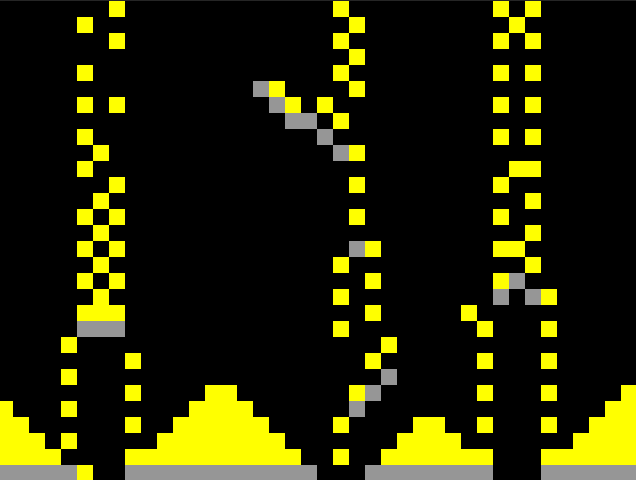
\includegraphics[width=.3\textwidth]{img/sable1.png}\hfill
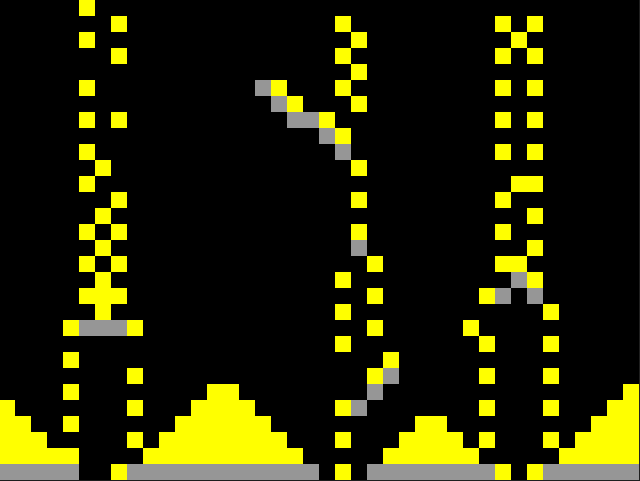
\includegraphics[width=.3\textwidth]{img/sable2.png}\hfill
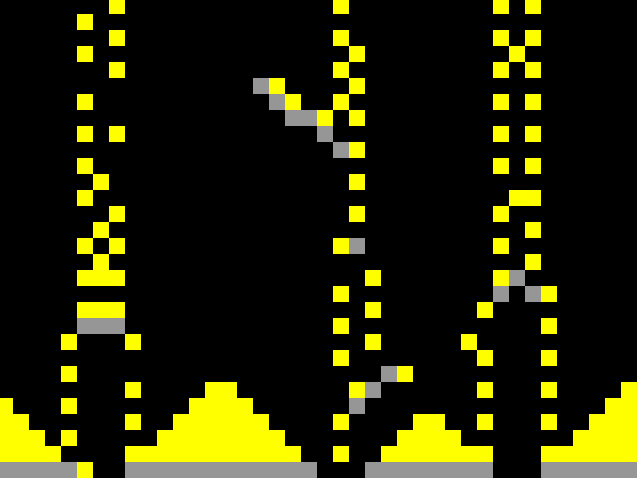
\includegraphics[width=.3\textwidth]{img/sable3.png}

\caption{Rendu achievement 2}
\label{fig:sable_disp}

\end{figure}

\newpage
\section*{Conclusion}
Le projet Sandwich a été l'occasion d'apprendre à utiliser des outils utiles pour la gestion de projet informatique, mais aussi comment s'organiser pour travailler en binôme sur des mêmes fichiers.\\
\indent Le projet a fait office de premier contact avec la programmation modulaire. Nous avons compris via ce projet les avantages que présente ce mode de fonctionnement. Cela nous a permis de séparer les programmes par fichier "thématique" (le monde, la file et les règles) rendant la compréhension des programmes plus simple que s'ils étaient tous regroupés en un même fichier. De plus, ce mode de fonctionnement permet de réutiliser dans plusieurs fichiers une même fonction sans la redéfinir. Par conséquent, lorsqu'on regroupe les programmes dans le fichier main.c contenant l'algorithme principal, cela permet de faire de l'abstraction, car les objets (file, monde, règles) sont manipulés via des fonctions dont les définitions se trouvent dans d'autres fichiers (world.c, queue.c, rule.c).
Du côté des outils de gestion de projet, nous nous sommes familiarisés avec l'utilisation de Git (pour travailler en parallèle) et d'un fichier Makefile (pour la compilation séparée). Ces deux outils étant utilisés très fréquemment, leur apprentissage lors de ce projet sera certainement mis à profit par la suite.\\
\indent Enfin, l'état final de notre projet nous satisfait, néanmoins certains points sont améliorables. Premièrement, bien que le travail fut généralement bien réparti, il nous est arrivé plusieurs fois de travailler à deux sur un même aspect. Deuxièmement, les tests sont quant à eux peu nombreux et auraient nécessité plus d'attention de notre part. Ces deux aspects constituent les points que nous devront améliorer lors de nos prochains projets.
\end{document}
